\documentclass{article}
\usepackage[margin=10mm]{geometry}
\usepackage{tikz}
\pagestyle{empty}
\begin{document}
\section*{row-style}

\begin{tikzpicture}[x=1mm,y=-1mm]
% 100mm × 80mm, light appearance
\path[opacity=0.25,fill={rgb,255:red,255;green,0;blue,0},draw={rgb,255:red,0;green,0;blue,0},line width=0.7mm,line cap=butt,line join=miter] (10,20) circle[radius=2mm];
\end{tikzpicture}

\newpage
\section*{empty-area}
\begin{tikzpicture}[x=1mm,y=-1mm]
% 100mm × 80mm, light appearance
\end{tikzpicture}

\newpage
\section*{heatmap-rectangle}

\begin{tikzpicture}[x=1mm,y=-1mm]
% 100mm × 80mm, light appearance
\path[fill={rgb,255:red,137;green,26;blue,26}] (10,20) rectangle ++(20,20);
\end{tikzpicture}

\newpage
\section*{vertical-rule}

\begin{tikzpicture}[x=1mm,y=-1mm]
% 100mm × 80mm, light appearance
\path[draw={rgb,255:red,137;green,26;blue,26},line width=0.3mm,line cap=butt,line join=miter,dash pattern=on 2mm off 1mm] (25,0) -- (25,80);
\end{tikzpicture}

\newpage
\section*{polar-point}

\begin{tikzpicture}[x=1mm,y=-1mm]
% 100mm × 100mm, light appearance
\path[fill={rgb,255:red,137;green,26;blue,26}] (100,50) circle[radius=2.2568mm];
\end{tikzpicture}

\newpage
\section*{top-axis}
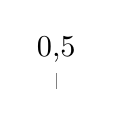
\begin{tikzpicture}[x=1mm,y=-1mm]
% 100mm × 80mm, light appearance
\path[draw={rgb,255:red,128;green,128;blue,128},line width=0.1mm,line cap=butt,line join=miter] (50,10) -- (50,8);
\node[anchor=center,text={rgb,255:red,0;green,0;blue,0},text opacity=1,rotate=0,align=left,font=\fontsize{11.2}{13.44}\selectfont] at (50,5) {0,5};
\end{tikzpicture}

\newpage
\section*{right-axis}
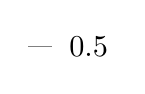
\begin{tikzpicture}[x=1mm,y=-1mm]
% 100mm × 80mm, light appearance
\path[draw={rgb,255:red,128;green,128;blue,128},line width=0.1mm,line cap=butt,line join=miter] (90,40) -- (93,40);
\node[anchor=west,text={rgb,255:red,0;green,0;blue,0},text opacity=1,rotate=0,align=left,font=\fontsize{11.2}{13.44}\selectfont] at (94,40) {0.5};
\end{tikzpicture}

\newpage
\section*{grid-only}
\begin{tikzpicture}[x=1mm,y=-1mm]
% 100mm × 80mm, light appearance
\path[draw={rgb,255:red,192;green,192;blue,192},line width=0.1mm,line cap=butt,line join=miter] (54,8) -- (54,66);
\end{tikzpicture}

\newpage
\section*{localized-annotation}

\begin{tikzpicture}[x=1mm,y=-1mm]
% 100mm × 80mm, light appearance
\node[anchor=west,text={rgb,255:red,0;green,128;blue,0},text opacity=1,rotate=0,align=left,font=\fontsize{9}{10.8}\selectfont] at (12,13) {Umsatz};
\end{tikzpicture}

\newpage
\section*{area-boundary}

\begin{tikzpicture}[x=1mm,y=-1mm]
% 100mm × 80mm, light appearance
\path[fill={rgb,255:red,137;green,26;blue,26}] (10,15) -- (20,10) -- (20,45) -- (10,35) -- cycle;
\end{tikzpicture}

\newpage
\section*{line-curve}
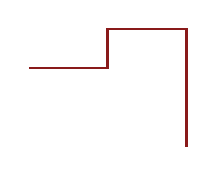
\begin{tikzpicture}[x=1mm,y=-1mm]
% 100mm × 80mm, light appearance
\path[draw={rgb,255:red,137;green,26;blue,26},line width=0.3mm,line cap=butt,line join=miter] (10,15) -- (20,15) -- (20,10) -- (30,10) -- (30,25);
\end{tikzpicture}

\newpage
\section*{link-curve}
\begin{tikzpicture}[x=1mm,y=-1mm]
% 100mm × 80mm, light appearance
\path[draw={rgb,255:red,137;green,26;blue,26},line width=0.3mm,line cap=butt,line join=miter] (10,15) .. controls (20,15) and (20,45) .. (30,45);
\end{tikzpicture}

\newpage
\section*{arc-center}

\begin{tikzpicture}[x=1mm,y=-1mm]
% 100mm × 80mm, light appearance
\path[fill={rgb,255:red,137;green,26;blue,26}] (50,20) arc[start angle=90,end angle=0,radius=20mm] -- (55,40) arc[start angle=0,end angle=90,radius=5mm] -- cycle;
\end{tikzpicture}

\newpage
\section*{rect-dimensions}

\begin{tikzpicture}[x=1mm,y=-1mm]
% 100mm × 80mm, light appearance
\path[fill={rgb,255:red,137;green,26;blue,26}] (5,10) rectangle ++(8,12);
\end{tikzpicture}

\newpage
\section*{horizontal-bar}

\begin{tikzpicture}[x=1mm,y=-1mm]
% 100mm × 80mm, light appearance
\path[fill={rgb,255:red,137;green,26;blue,26}] (0,10) rectangle ++(35,4);
\end{tikzpicture}

\newpage
\section*{circle-radius}

\begin{tikzpicture}[x=1mm,y=-1mm]
% 100mm × 80mm, light appearance
\path[fill={rgb,255:red,137;green,26;blue,26}] (10,20) circle[radius=7mm];
\end{tikzpicture}

\newpage
\section*{symbol-shape}

\begin{tikzpicture}[x=1mm,y=-1mm]
% 100mm × 80mm, light appearance
\path[fill={rgb,255:red,137;green,26;blue,26}] (0,-5.8857) -- (3.3981,0) -- (0,5.8857) -- (-3.3981,0) -- cycle;
\end{tikzpicture}

\newpage
\section*{band-boundary}

\begin{tikzpicture}[x=1mm,y=-1mm]
% 100mm × 80mm, light appearance
\path[fill={rgb,255:red,137;green,26;blue,26}] (10,15) -- (20,10) -- (20,45) -- (10,35) -- cycle;
\end{tikzpicture}

\newpage
\section*{polygon-points}
\begin{tikzpicture}[x=1mm,y=-1mm]
% 100mm × 80mm, light appearance
\path[fill={rgb,255:red,137;green,26;blue,26}] (1,2) -- (3,4) -- (5,6) -- cycle;
\end{tikzpicture}

\newpage
\section*{path-curve}
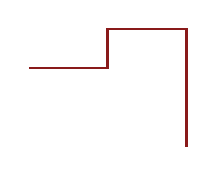
\begin{tikzpicture}[x=1mm,y=-1mm]
% 100mm × 80mm, light appearance
\path[draw={rgb,255:red,137;green,26;blue,26},line width=0.3mm,line cap=butt,line join=miter] (10,15) -- (20,15) -- (20,10) -- (30,10) -- (30,25);
\end{tikzpicture}

\newpage
\section*{trail-width}

\begin{tikzpicture}[x=1mm,y=-1mm]
% 100mm × 80mm, light appearance
\path[draw={rgb,255:red,137;green,26;blue,26},line width=2mm,line cap=butt,line join=miter] (10,15) -- (20,10);
\path[draw={rgb,255:red,137;green,26;blue,26},line width=4mm,line cap=butt,line join=miter] (20,10) -- (30,25);
\end{tikzpicture}

\newpage
\section*{ribbon-geometry}

\begin{tikzpicture}[x=1mm,y=-1mm]
% 100mm × 80mm, light appearance
\path[fill={rgb,255:red,137;green,26;blue,26}] (0,-20) arc[start angle=90,end angle=61.3521,radius=20mm] .. controls (3.1962,-5.8506) and (5.6098,-3.602) .. (16.8294,-10.806) arc[start angle=32.7042,end angle=4.0563,radius=20mm] .. controls (6.65,-0.4716) and (0,-6.6667) .. (0,-20) -- cycle;
\end{tikzpicture}

\newpage
\section*{pie-layout}
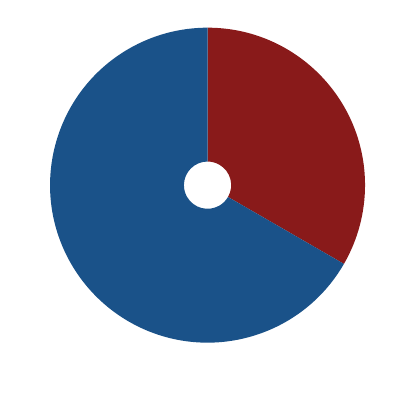
\begin{tikzpicture}[x=1mm,y=-1mm]
% 100mm × 80mm, light appearance
\path[fill={rgb,255:red,137;green,26;blue,26}] (50,20) arc[start angle=90,end angle=-30,radius=20mm] -- (52.5981,41.5) arc[start angle=-30,end angle=90,radius=3mm] -- cycle;
\path[fill={rgb,255:red,26;green,82;blue,137}] (67.3205,50) arc[start angle=-30,end angle=-150,radius=20mm] arc[start angle=-150,end angle=-270,radius=20mm] -- (50,37) arc[start angle=-270,end angle=-150,radius=3mm] arc[start angle=-150,end angle=-30,radius=3mm] -- cycle;
\end{tikzpicture}

\newpage
\section*{text-style}

\begin{tikzpicture}[x=1mm,y=-1mm]
% 100mm × 80mm, light appearance
\node[anchor=east,text={rgb,255:red,0;green,0;blue,255},text opacity=0.5,rotate=-15,align=left,font=\fontsize{9}{10.8}\selectfont] at (10,15) {Cost \& tax 20\%\_\#\$\{\}\textasciicircum{}\textasciitilde{}\textbackslash{}};
\end{tikzpicture}

\newpage
\section*{encoded-color-scale}

\begin{tikzpicture}[x=1mm,y=-1mm]
% 100mm × 80mm, light appearance
\path[fill={rgb,255:red,0;green,255;blue,0}] (10,20) circle[radius=2.2568mm];
\end{tikzpicture}

\newpage
\section*{line-detail-order}
\begin{tikzpicture}[x=1mm,y=-1mm]
% 100mm × 80mm, light appearance
\path[draw={rgb,255:red,137;green,26;blue,26},line width=0.3mm,line cap=butt,line join=miter] (10,15) -- (20,10);
\path[draw={rgb,255:red,137;green,26;blue,26},line width=0.3mm,line cap=butt,line join=miter] (30,20) -- (40,30);
\end{tikzpicture}

\newpage
\section*{row-line-styles}
\begin{tikzpicture}[x=1mm,y=-1mm]
% 100mm × 80mm, light appearance
\path[opacity=0.2,draw={rgb,255:red,255;green,0;blue,0},line width=0.3mm,line cap=butt,line join=miter] (1,2) -- (3,4);
\path[opacity=0.5,draw={rgb,255:red,0;green,255;blue,0},line width=0.3mm,line cap=butt,line join=miter] (3,4) -- (5,6);
\end{tikzpicture}

\newpage
\section*{point-gap}

\begin{tikzpicture}[x=1mm,y=-1mm]
% 100mm × 80mm, light appearance
\path[fill={rgb,255:red,137;green,26;blue,26}] (1,2) circle[radius=2.2568mm];
\path[fill={rgb,255:red,137;green,26;blue,26}] (5,6) circle[radius=2.2568mm];
\end{tikzpicture}

\newpage
\section*{line-gap}
\begin{tikzpicture}[x=1mm,y=-1mm]
% 100mm × 80mm, light appearance
\path[draw={rgb,255:red,137;green,26;blue,26},line width=0.3mm,line cap=butt,line join=miter] (1,2) -- cycle (5,6) -- cycle;
\end{tikzpicture}

\newpage
\section*{normalized-cartesian}

\begin{tikzpicture}[x=1mm,y=-1mm]
% 100mm × 80mm, light appearance
\path[fill={rgb,255:red,137;green,26;blue,26}] (25,20) circle[radius=2.2568mm];
\end{tikzpicture}

\newpage
\section*{transpose-cartesian}

\begin{tikzpicture}[x=1mm,y=-1mm]
% 100mm × 80mm, light appearance
\path[fill={rgb,255:red,137;green,26;blue,26}] (75,60) circle[radius=2.2568mm];
\end{tikzpicture}

\newpage
\section*{left-axis}

\begin{tikzpicture}[x=1mm,y=-1mm]
% 100mm × 80mm, light appearance
\path[draw={rgb,255:red,128;green,128;blue,128},line width=0.1mm,line cap=butt,line join=miter] (10,40) -- (7,40);
\node[anchor=east,text={rgb,255:red,0;green,0;blue,0},text opacity=1,rotate=0,align=left,font=\fontsize{11.2}{13.44}\selectfont] at (6,40) {0.5};
\end{tikzpicture}

\newpage
\section*{bottom-band-axis}
\begin{tikzpicture}[x=1mm,y=-1mm]
% 100mm × 80mm, light appearance
\path[draw={rgb,255:red,128;green,128;blue,128},line width=0.1mm,line cap=butt,line join=miter] (30,70) -- (30,72);
\node[anchor=center,text={rgb,255:red,0;green,0;blue,0},text opacity=1,rotate=0,align=left,font=\fontsize{11.2}{13.44}\selectfont] at (30,75) {a};
\path[draw={rgb,255:red,128;green,128;blue,128},line width=0.1mm,line cap=butt,line join=miter] (70,70) -- (70,72);
\node[anchor=center,text={rgb,255:red,0;green,0;blue,0},text opacity=1,rotate=0,align=left,font=\fontsize{11.2}{13.44}\selectfont] at (70,75) {b};
\end{tikzpicture}

\newpage
\section*{legend-color}
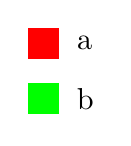
\begin{tikzpicture}[x=1mm,y=-1mm]
% 100mm × 80mm, light appearance
\path[fill={rgb,255:red,255;green,0;blue,0}] (70,18) rectangle ++(4,4);
\node[anchor=west,text={rgb,255:red,0;green,0;blue,0},text opacity=1,rotate=0,align=left,font=\fontsize{11.2}{13.44}\selectfont] at (75,20) {a};
\path[fill={rgb,255:red,0;green,255;blue,0}] (70,25) rectangle ++(4,4);
\node[anchor=west,text={rgb,255:red,0;green,0;blue,0},text opacity=1,rotate=0,align=left,font=\fontsize{11.2}{13.44}\selectfont] at (75,27) {b};
\end{tikzpicture}

\newpage
\section*{annotation-shapes}
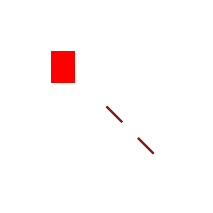
\begin{tikzpicture}[x=1mm,y=-1mm]
% 100mm × 80mm, light appearance
\path[fill={rgb,255:red,255;green,0;blue,0}] (1,2) rectangle ++(3,4);
\path (5,6) circle[radius=7mm];
\path[draw={rgb,255:red,137;green,26;blue,26},line width=0.3mm,line cap=butt,line join=miter] (8,9) -- (10,11);
\path[draw={rgb,255:red,137;green,26;blue,26},line width=0.3mm,line cap=butt,line join=miter] (12,13) -- (14,15);
\path (16,17) circle[radius=2mm];
\end{tikzpicture}

\newpage
\section*{localized-title}

\begin{tikzpicture}[x=1mm,y=-1mm]
% 100mm × 80mm, light appearance
\node[anchor=center,text={rgb,255:red,0;green,0;blue,0},text opacity=1,rotate=0,align=left,font=\fontsize{12.8}{15.36}\selectfont] at (50,4) {Revenue};
\end{tikzpicture}

\newpage
\section*{clip-and-dash}
\begin{tikzpicture}[x=1mm,y=-1mm]
% 100mm × 80mm, light appearance
\begin{scope}
\clip (0,0) rectangle (100,80);
\path[draw={rgb,255:red,255;green,0;blue,0},line width=0.3mm,line cap=round,line join=bevel,dash pattern=on 2mm off 1mm] (10,15) -- (20,10);
\end{scope}
\end{tikzpicture}

\newpage
\section*{normalized-rect}

\begin{tikzpicture}[x=1mm,y=-1mm]
% 100mm × 80mm, light appearance
\path[fill={rgb,255:red,137;green,26;blue,26}] (20,56) -- (40,56) -- (40,32) -- (20,32) -- cycle;
\end{tikzpicture}

\newpage
\section*{normalized-rule}

\begin{tikzpicture}[x=1mm,y=-1mm]
% 100mm × 80mm, light appearance
\path[draw={rgb,255:red,137;green,26;blue,26},line width=0.3mm,line cap=butt,line join=miter] (0,60) -- (100,60);
\end{tikzpicture}

\newpage
\section*{polar-rect}

\begin{tikzpicture}[x=1mm,y=-1mm]
% 100mm × 80mm, light appearance
\path[fill={rgb,255:red,137;green,26;blue,26}] (50,20) arc[start angle=90,end angle=0,radius=20mm] -- (60,40) arc[start angle=0,end angle=90,radius=10mm] -- cycle;
\end{tikzpicture}

\newpage
\section*{full-circle-path}

\begin{tikzpicture}[x=1mm,y=-1mm]
% 100mm × 80mm, light appearance
\path[fill={rgb,255:red,137;green,26;blue,26}] (50,30) arc[start angle=90,end angle=-90,radius=10mm] arc[start angle=-90,end angle=-270,radius=10mm] -- cycle;
\end{tikzpicture}

\newpage
\section*{geographic-point}

\begin{tikzpicture}[x=1mm,y=-1mm]
% 100mm × 80mm, light appearance
\path[fill={rgb,255:red,137;green,26;blue,26}] (75,40) circle[radius=2.2568mm];
\end{tikzpicture}

\newpage
\end{document}